\documentclass[aspectratio=169]{beamer}
%\setbeameroption{show notes on second screen=right} % Both
\setbeameroption{hide notes} % Only slides
%\setbeameroption{show only notes} % Only notes
% Theme choice:
\usetheme{Boadilla}
\usepackage{tikz-feynman}
\usepackage{array}
\usepackage{animate}
\usepackage{amsmath}
\usepackage{cancel}
\usepackage{multicol}
\usepackage{physics}
\usepackage{xcolor}
\usepackage{graphicx,subcaption}
\usepackage{amssymb}
\usepackage{hyperref}
%\hypersetup{colorlinks = true,linkcolor = black,filecolor= black,urlcolor= black}
\usepackage{cancel}
\usepackage{subcaption}
\usepackage{comment}
\usepackage[backend=bibtex,bibencoding=utf8,style=authortitle,citestyle=authortitle]{biblatex}
\addbibresource{library}
\AtEveryBibitem{%
	\clearname{translator}%
	\clearlist{publisher}%
	\clearfield{pagetotal}%
}
\usepackage{xparse}

\usepackage[toc,page]{appendix}
\author{Tran Khoi Nguyen}
% Title page details: 
\author[Presenter: Tran Khoi Nguyen]{{\textit{Presenter}} \\
	Tran Khoi Nguyen \inst{1} \\
	{\and} \\
	{\textit{Supervisors}} \\
	Dr. Huynh Thanh Duc \inst{2}}
\institute[HCMUS]{\inst{1} University of Science, Ho Chi Minh city\and %
	\inst{2} Institute of Applied Mechanics and Informatics}
% Title page details: 
\title[Hofstadter butterfly of TMD]{Hofstadter butterfly in transistion metal dichalcogenide monolayers}
	
\date{Jul, 2025}
\logo{\includegraphics[height=0.9cm]{pic/logo1.png}\vspace*{-.055\paperheight}\hspace*{.85\paperwidth}}

\begin{document}
	\setbeamertemplate{logo}{}
	\begin{frame}
		\titlepage
		\note{Good day, teachers and fellow students. Now is my turn to present my work, on the "Calculation of the linear absorption spectrum of MoS2".}
	\end{frame}
	\logo{}
	\begin{frame}{Table of Contents}
		\tableofcontents
		\note{note text}
	\end{frame}
	\section{Overview}
	\begin{frame}{Overview}
		Group VI-B Transition Metal Dichalcogenides (TMD) are compound semiconductors of the type $MX_2$
		\begin{figure}
			\begin{subfigure}[b]{0.495\textwidth}
				\centering
				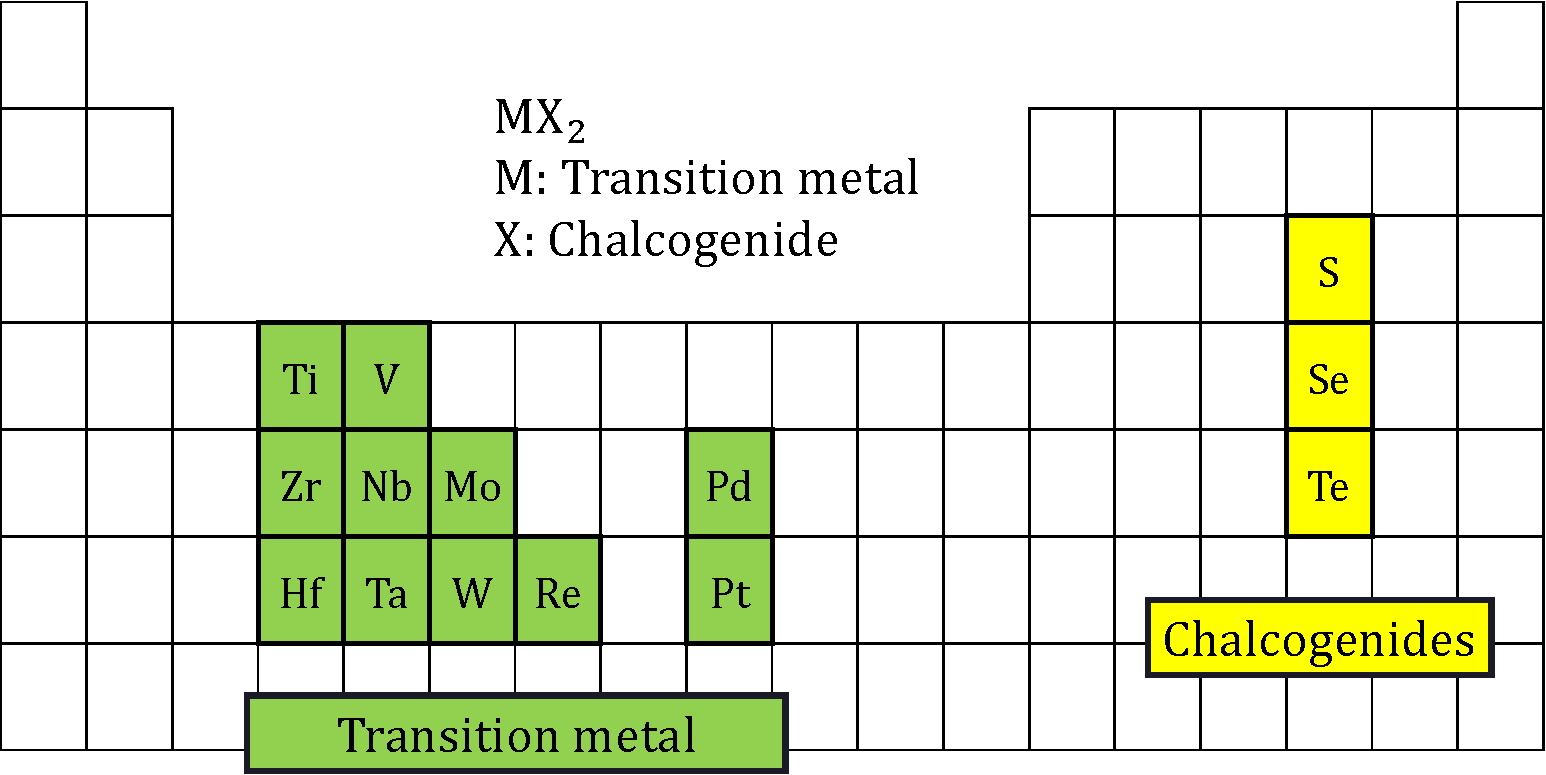
\includegraphics[width=1.0\linewidth]{pic/periodictable.pdf}
			\end{subfigure}
			\begin{subfigure}[b]{0.495\textwidth}
				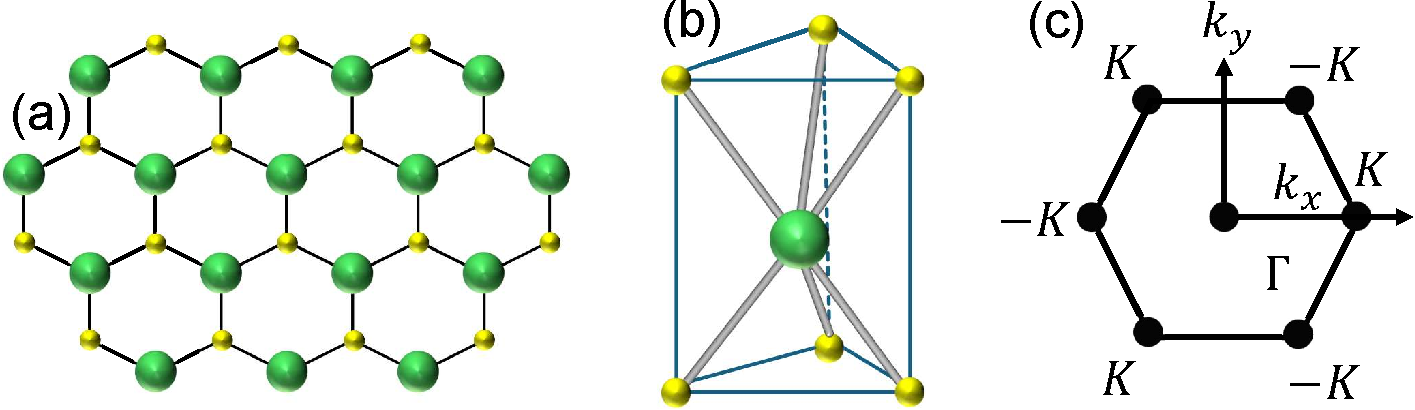
\includegraphics[width=1.0\linewidth]{pic/lattice_crop.pdf}
			\end{subfigure}
			\caption{Transition metal dichalcogenides compound. Top view of monolayer $MX_{2}$. The large sphere is $M$ atom and the small sphere is $X$.}
		\end{figure}
	\end{frame}
	\section{Method}
	\subsection{Three-band tigh-binding model without magnetic field}
	\begin{frame}{Transition Metal Dichalcogenides Monolayers}
		\begin{itemize}
			\item One $\color{green}M$ layer sandwiched by two $\color{yellow}X$ layers as show in top view (a) and side view (b)
			\item They have the inverse 
		\end{itemize}
	\end{frame}
	\begin{frame}
		\begin{itemize}
			\item 
		\end{itemize}
	\end{frame}
	\subsection{Three-band tigh-binding model under a magnetic field}
	\begin{frame}{Three-band tigh-binding model under a magnetic field}
		\begin{figure}
			\centering
			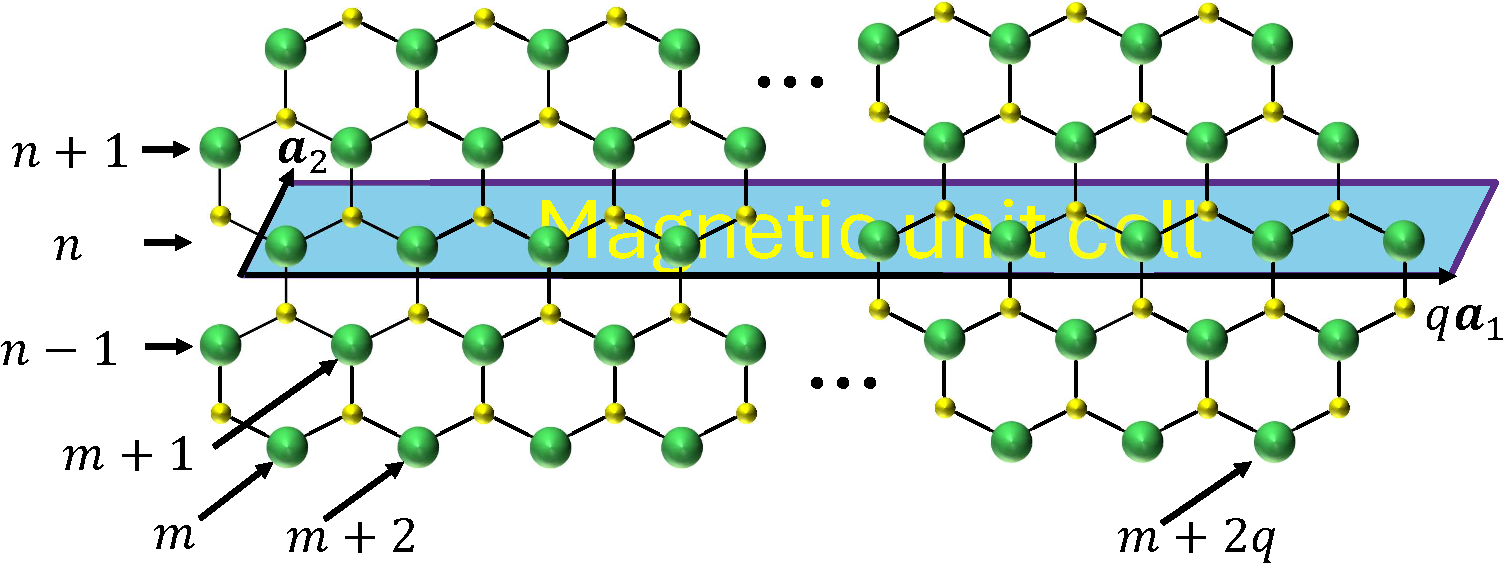
\includegraphics[width=0.85\textwidth,height=0.35\linewidth]{pic/magneticUC_cut.pdf}
			\caption{\label{fig:Mag UC} Magnetic unit cell for TMD monolayers.}
		\end{figure}
	\end{frame}
	\subsection{Landau levels}
	\begin{frame}{Landau levels}
		\note{note text}
	\end{frame}
	\subsection{Quantum Hall effect}
	\begin{frame}{Classical Hall effect}
		\note{note text}
	\end{frame}
	\section{Summary and Outlook}
	\begin{frame}
		\begin{block}{Summary:}
			\begin{itemize}
				\item We confirm the Hofstadter butterfly in this model corrected compared to previous study.\\
				\item From three-band TB + magnetic field $\to$ QHE.
			\end{itemize}
		\end{block}
		\begin{exampleblock}{Further research:}
			\begin{itemize}
				\item High Harmonic Generation
				\item High-order Side-band Generation
				\item Photovoltaic effect
			\end{itemize}
		\end{exampleblock}
		\begin{multicols}{2}
			\begin{center}
				\null\vfill
				Thank you for your listening.
				\null\vfill
			\end{center}\columnbreak
		\end{multicols}
		\note[item]{So far, we have used the three-band tight-binding model and semiconductor Bloch equations to calculate the linear absorption spectrum. We confirm that this model matches the results with the experiment data and also predicts smaller exciton peaks.}
		\note[item]{For further results, we can include the many-body interaction in calculating other phenomena for a realistic picture of TMD's properties.}
	\end{frame}
\end{document}